\begin{surferPage}[Beşgil (15 Gaga)]{15 Gagalı Bir Beşgil}
Derecesi  $5$ olan bu yüzey (beşgil)  $A_2$ türünden $15$ tekilliğe sahip; bu tekilliklere gaga (İng. cusp) diyoruz. Bu beşgil ve ilişkili birkaç yüzey daha  Oliver Labs'ın 2005 makalesinde verilmiştir.
Buradaki gagalardan beş tanesi diğer on tanesinden farklı görünüyor.
Bu beş taneye  $A_2^{++}$ tekilliği, diğerlerine $A_2^{+-}$ tekilliği deniyor.
% (see  the gallery on simple singularities for more info):

     \vspace*{-0.3em}
    \begin{center}
      \begin{tabular}{c@{\qquad}c}
        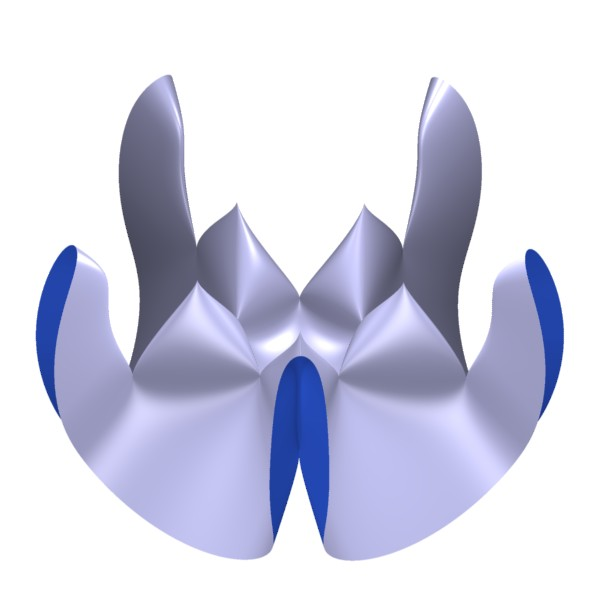
\includegraphics[height=1.2cm]{./../../common/images/dessins_quint_15a2}
        &
        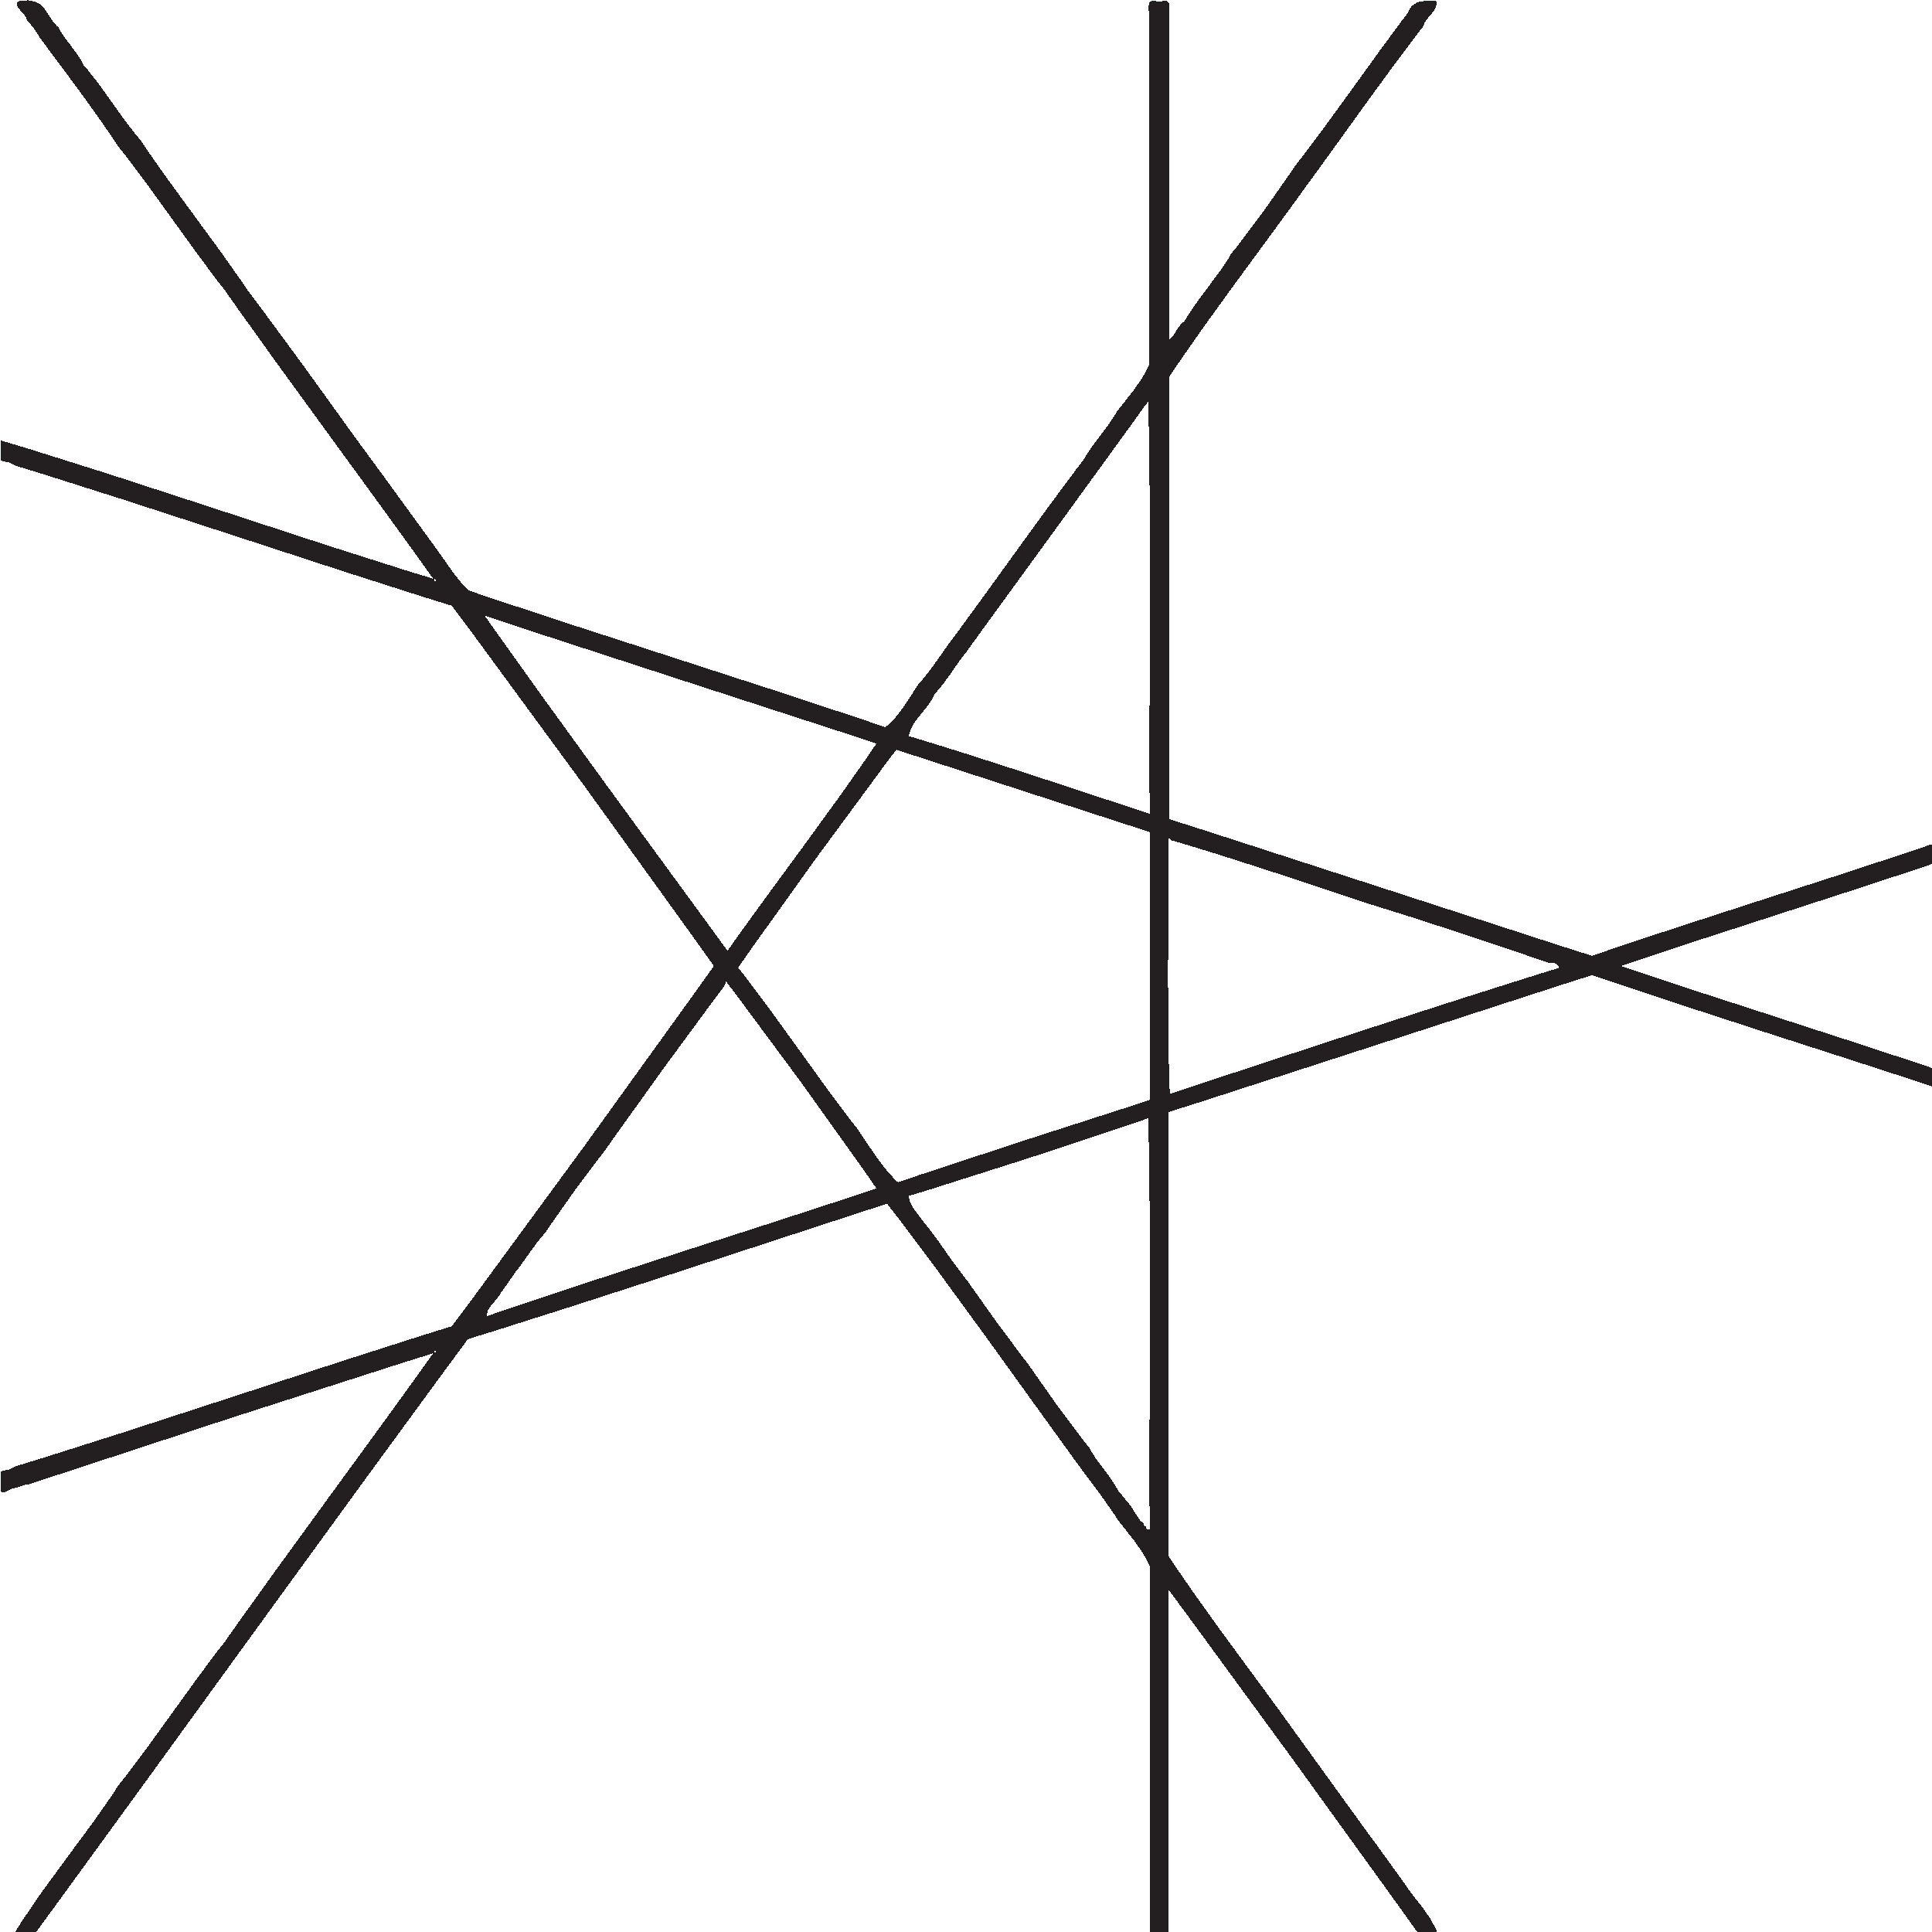
\includegraphics[height=1.2cm]{./../../common/images/rp5.pdf}
      \end{tabular}
    \end{center}
    \vspace*{-0.3em}    
    
Bu yüzeyin denklemi    $S_5(x,y) + t(z)=0$.
Burada $S_5(x,y)$  bir düzgün beşgenin simetrilerini veren doğrular çarpımı  (sağ resim) ve $t(z)$ daha önce birkaç kez söz ettiğimiz Çebişev polinomlarıdır.

 $15$ gagalı başka bir beşgil Wolf Barth tarafından inşa edilmiştir (solda); 
orta resimde görüleceği gibi bu yüzey  Clebsch'in Kübiği (sağda) ile ilişkilidir:

    \vspace*{-0.3em}
    \begin{center}
      \begin{tabular}{c@{\quad}c@{\quad}c}
        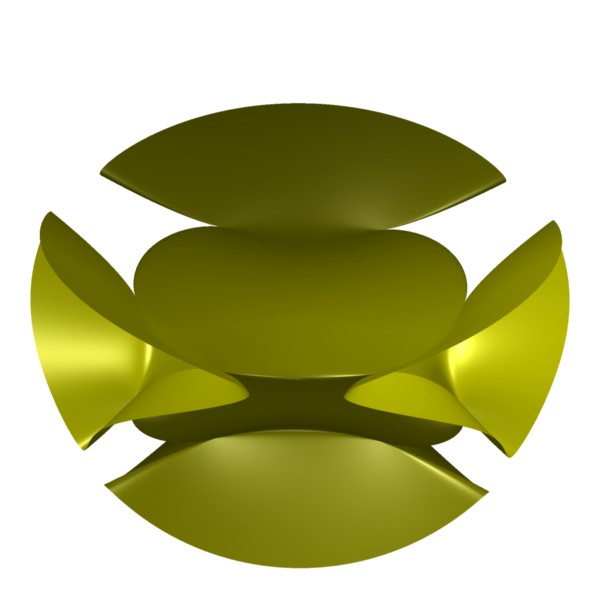
\includegraphics[height=1.2cm]{./../../common/images/barthquintic_green}
        &
        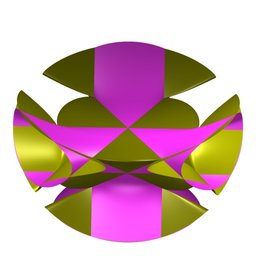
\includegraphics[height=1.2cm]{./../../common/images/barthquintic_clebschcubic}
        &
        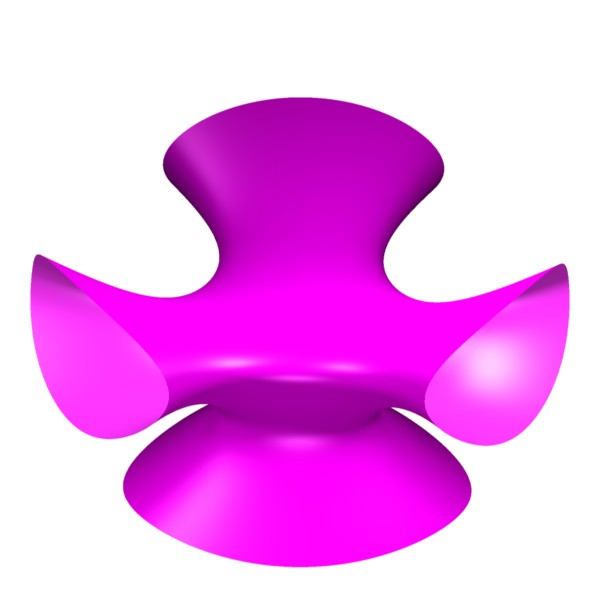
\includegraphics[height=1.2cm]{./../../common/images/clebschcubic_pink}
      \end{tabular}
    \end{center}
    \vspace*{-0.3em}
\end{surferPage}
